% Provenance (never printed): see sources/outline_sources.md (Year 2: the solar nebula
% and the condensation sequence; planetesimals and embryos; chondrites, achondrites and
% irons; the age of the Solar System; differentiation of planets). Curves from
% figdata/bachelor-2/nebula.py, condensation.py, al26.py, meteorites.py; exercise and
% problem values in the Book 4 scratch calculator calc/ch02.py.
\chapter{La formación de los planetas y los meteoritos}\label{ch:b2:planet-formation-meteorites}

Cada año entran en la atmósfera terrestre unas quince mil toneladas de polvo
del espacio; la mayor parte se quema o se deposita como esférulas microscópicas, y de vez
en cuando cae una piedra del tamaño de un puño con una bola de fuego y un estampido sónico.
La mayoría de esas piedras son fragmentos de asteroides, y muchas apenas han cambiado
desde que se formaron. Si se corta una y se pule, muestra esférulas milimétricas
de roca que estuvo fundida, granos blancos irregulares de minerales de calcio y
aluminio y escamas de metal, todo ello sujeto en un cemento oscuro de grano fino. Los granos
blancos son los sólidos más antiguos del sistema solar: los isótopos del plomo les dan
4567 millones de años. Un segundo reloj, la desintegración de un isótopo radiactivo del
aluminio desaparecido hace mucho, data los demás componentes con respecto a
ellos con una precisión de una fracción de millón de años. Este capítulo sigue el disco del
capítulo anterior mientras se convierte en planetas: qué sólidos condensan del gas que
se enfría, y dónde; cómo el polvo crece hasta cuerpos de kilómetros y luego
hasta planetas; qué son los \omterm{def:b2:planet-formation-meteorites:fall-find}{meteoritos}, y cómo datan esos acontecimientos; y por qué
algunos de los primeros cuerpos se fundieron y formaron núcleos de hierro mientras otros quedaron tal como se
habían formado.
% ledger: rojas21:flux, lugaro:cai, gail:meteorites

\begin{recall}
Las estrellas jóvenes están rodeadas de \omterm{def:b2:ism-star-formation:disc}{discos protoplanetarios}, que desaparecen en unos
pocos millones de años; un grano iluminado a la distancia $r$ de una estrella de
luminosidad $L$ se estabiliza a $T = \bigl(L/(16\pi\sigma r^2)\bigr)^{1/4}$
(\cref{ch:b2:ism-star-formation}). Los asteroides son los cuerpos pequeños, rocosos o metálicos,
del sistema solar, la mayoría de los cuales orbitan entre Marte y Júpiter (volumen de primer
año). Un núcleo radiactivo se desintegra con la probabilidad $\lambda$ por unidad de
tiempo: $N = N_0 e^{-\lambda t}$; el periodo de semidesintegración es $\ln 2/\lambda$, y la vida
media $\tau = 1/\lambda$ (física). En un sistema cerrado, las muestras cogenéticas de
distintas razones padre/hija se alinean en una recta, la isócrona, cuya
pendiente da la edad y cuya ordenada en el origen es la razón inicial (volumen de primer año).
Calentar una masa $m$ de capacidad calorífica específica $c$ en $\Delta T$ requiere la energía
$mc\,\Delta T$ (física).
\end{recall}

\section{La nebulosa solar}

\begin{definition}[Nebulosa solar]\label{def:b2:planet-formation-meteorites:nebula}
La \emph{nebulosa solar}\index{nebulosa solar} es el \omterm{def:b2:ism-star-formation:disc}{disco protoplanetario} de gas
y polvo que rodeaba al Sol joven y del que se formaron los planetas, sus
satélites, los asteroides y los cometas.
\end{definition}

¿Cuánta materia contenía? Un límite inferior lo dan los propios planetas.
Si se añade a cada planeta el hidrógeno y el helio necesarios para darle la composición del
Sol y se reparte el resultado sobre un anillo centrado en su órbita, la densidad
superficial, la masa por unidad de área del disco, disminuye con la distancia al
Sol. Esta reconstrucción es la \emph{nebulosa solar de masa
mínima}\index{nebulosa solar de masa mínima}. En una versión muy usada la densidad
superficial del gas es
\[
  \Sigma_g = \qty{2200}{g.cm^{-2}}\left(\frac{r}{\qty{1}{au}}\right)^{-3/2},
\]
y la de los sólidos $\Sigma_p = \qty{33}{g.cm^{-2}}\,Z_{\mathrm{rel}}\,
(r/\qty{1}{au})^{-3/2}$, donde $Z_{\mathrm{rel}}$ es la fracción de la materia
condensable que es realmente sólida: $0.33$ donde solo han condensado la roca y el metal,
unos $0.78$ donde se les ha unido el hielo de agua, y $1$ más allá del lugar
donde se congela el metano. Las cifras son inciertas: el contenido en elementos pesados de
Júpiter solo se conoce dentro de un factor cuatro, y los planetas no tienen por qué haberse
formado donde orbitan ahora.
% ledger: cy10:mmsn

\begin{proposition}[Masa de un disco]\label{prop:b2:planet-formation-meteorites:disc-mass}
Un disco de densidad superficial $\Sigma(r) = \Sigma_1 (r/r_1)^{-3/2}$ contiene, dentro
del radio $R$, la masa
\[
  M(R) = 4\pi\Sigma_1 r_1^2 \left(\frac{R}{r_1}\right)^{1/2}.
\]
La mayor parte de la masa está lejos: duplicar el radio añade un \qty{41}{\percent} a
la masa.
\end{proposition}

\begin{proof}
Un anillo de radio $r$ y anchura $\mathrm dr$ tiene el área $2\pi r\,\mathrm dr$, de modo que
\[
  M(R) = \int_0^R 2\pi r\,\Sigma_1 \left(\frac{r}{r_1}\right)^{-3/2}\mathrm dr
       = 2\pi\Sigma_1 r_1^{3/2}\int_0^R r^{-1/2}\,\mathrm dr
       = 4\pi\Sigma_1 r_1^{3/2} R^{1/2},
\]
que es la fórmula; la integral converge en $r = 0$. Duplicar $R$
multiplica $M$ por $\sqrt 2 = 1.41$.
\end{proof}

Con $\Sigma_1 = \qty{2.2e4}{kg.m^{-2}}$ en $r_1 = \qty{1}{au}$, la nebulosa de masa
mínima contiene $0.03$ masas solares dentro de \qty{100}{au} (\cref{exo:b2:planet-formation-meteorites:5}). Los discos
observados alrededor de estrellas de un millón de años, pesados por el brillo milimétrico de
su polvo, contienen \numrange{0.001}{0.1} masas solares: la nebulosa de masa mínima
encaja sin dificultad entre ellos.
% ledger: cy10:mmsn

Casi toda esta masa es gas que nunca condensará. El Sol nació
con una fracción másica de hidrógeno $X_0 = 0.711$, de helio $Y_0 = 0.274$ y de
todos los elementos más pesados juntos solo $Z_0 = 0.0149$. Enfriar un gas de esta
composición hasta que se haya congelado todo lo que puede congelarse convierte en sólidos solo
el \qty{1.5}{\percent} de su masa: un \qty{0.49}{\percent} de roca y
metal, y un \qty{1.0}{\percent} de hielos de agua, metano y amoniaco, del que el hielo de agua
por sí solo es el \qty{0.57}{\percent}. Todos los planetas rocosos, y los núcleos de los
gigantes, se construyeron a partir de esta pequeña fracción.
% ledger: lodders:protosolar, lodders:condensates

La temperatura del disco decide qué es sólido y dónde. Un disco calentado solo por
su estrella, un disco \emph{pasivo}, es templado en su superficie, donde los granos ven
directamente la estrella (la proposición del \cref{ch:b2:ism-star-formation}), y
mucho más frío en su plano medio, que solo recibe el infrarrojo reemitido por
esos granos de superficie. Para una estrella joven de una masa solar, un modelo de un disco así
da la temperatura del plano medio
\[
  T = \qty{120}{K}\left(\frac{r}{\qty{1}{au}}\right)^{-3/7}.
\]
La acreción de gas a través del disco, que libera energía gravitatoria, calienta más
el plano medio, sobre todo al principio y cerca de la estrella (figura siguiente).
% ledger: cy10:passive

\begin{omfigure}
\begin{tikzpicture}
\begin{axis}[omrecord, width=0.82\linewidth, height=6.2cm, xmode=log, ymode=log,
  xmin=0.1, xmax=100, ymin=10, ymax=1000,
  xlabel={distancia a la estrella $r$ (au)}, ylabel={temperatura (K)},
  tick label style={font=\scriptsize}, label style={font=\small},
  legend pos=north east, legend style={font=\scriptsize, draw=black!30}]
\addplot[thick, red!70!black] table[x=r_au, y=T_grain] {figdata/out/bachelor-2-nebula-temp.dat};
\addlegendentry{granos bajo luz estelar directa}
\addplot[thick, blue!70!black] table[x=r_au, y=T_mid] {figdata/out/bachelor-2-nebula-temp.dat};
\addlegendentry{plano medio de un disco pasivo}
\addplot[black!50, densely dashed, domain=0.1:100, samples=2] {182};
\addplot[black!50, densely dashed, domain=0.1:100, samples=2] {41};
\node[font=\scriptsize, anchor=south east] at (axis cs:95,182) {hielo de agua, \qty{182}{K}};
\node[font=\scriptsize, anchor=north west] at (axis cs:0.46,41) {hielo de metano, \qty{41}{K}};
\draw[blue!70!black, -latex] (axis cs:0.38,25) -- (axis cs:0.38,175);
\node[font=\scriptsize, blue!70!black, anchor=north] at (axis cs:0.38,25) {\qty{0.4}{au}};
\draw[red!70!black, -latex] (axis cs:2.34,25) -- (axis cs:2.34,175);
\node[font=\scriptsize, red!70!black, anchor=north] at (axis cs:2.34,25) {\qty{2.3}{au}};
\end{axis}
\end{tikzpicture}

\par\smallskip{\small Dos temperaturas de un disco alrededor de una estrella de una luminosidad solar.
Rojo: un grano negro bajo luz estelar directa (\cref{ch:b2:ism-star-formation}). Azul: el
plano medio de un disco pasivo alrededor de una estrella joven de masa solar, protegido de la luz
directa. El hielo de agua es estable por debajo de \qty{182}{K}: las flechas marcan dónde cada curva
cruza esa línea. La \omterm{def:b2:planet-formation-meteorites:snow-line}{línea de nieve} real estaba entre esos límites y se desplazó a medida que el disco
evolucionaba. Datos: Chiang y Youdin (2010); Lodders (2003).}
% ledger: cy10:passive, lodders:phases, cy10:mmsn, sun:L, const:sigma
\end{omfigure}

\section{La secuencia de condensación}

Imagínese el gas de la nebulosa, cerca del Sol joven, lo bastante caliente para que todos los
elementos estén en forma de vapor, y déjese enfriar con la lentitud suficiente para que el gas y los sólidos
permanezcan en equilibrio químico. A medida que baja la temperatura, cada elemento
abandona a su vez el gas por un sólido, ya sea como compuesto propio o
disuelto en un sólido que ya se ha formado.

\begin{definition}[Temperatura de condensación, secuencia de condensación]
\label{def:b2:planet-formation-meteorites:condensation}
La \emph{temperatura de condensación}\index{temperatura de condensación} de un
elemento en un gas que se enfría, de composición y presión dadas, es la temperatura
a la que la mitad de él ha pasado a sólidos en equilibrio químico (la
\emph{temperatura de condensación al 50 por ciento}; la temperatura a la que aparece su primer
sólido es la temperatura de \emph{aparición}). La
\emph{secuencia de condensación}\index{secuencia de condensación} es el orden en que
aparecen los elementos y sus compuestos sólidos a medida que el gas se enfría.
\end{definition}

Los cálculos para un gas de composición solar se hacen a una presión total de
$10^{-4}$ bar, típica de la nebulosa cerca de \qty{1}{au}. Los primeros sólidos son
óxidos de aluminio y de calcio (tabla siguiente), que se forman hacia
\qty{1700}{K}; el grueso de la materia formadora de rocas, el silicato de magnesio y
el hierro metálico, condensa cerca de \qty{1350}{K}; el sulfuro de hierro espera hasta
\qty{704}{K}, y el hielo de agua hasta \qty{182}{K}.
% ledger: lodders:phases

\begin{table}[h]
\centering
\small
\begin{tabular}{lll}
\hline
sólido & fórmula & aparece a (K)\\
\hline
corindón & \ce{Al2O3} & 1677\\
hibonita & \ce{CaAl12O19} & 1659\\
perovskita & \ce{CaTiO3} & 1593\\
espinela & \ce{MgAl2O4} & 1397\\
metal hierro--níquel & \ce{Fe}, con \ce{Ni}, \ce{Co}, \ce{Cr} & 1357\\
forsterita & \ce{Mg2SiO4} & 1354\\
schreibersita & \ce{Fe3P} & 1248\\
troilita & \ce{FeS} & 704\\
magnetita & \ce{Fe3O4} & 371\\
hielo de agua & \ce{H2O} & 182\\
hidrato de amoniaco & \ce{NH3.H2O} & 131\\
clatrato de metano & \ce{CH4.7H2O} & 78\\
\hline
\end{tabular}
\caption{La \omterm{def:b2:planet-formation-meteorites:condensation}{secuencia de condensación} de un gas de composición del sistema solar a
$10^{-4}$ bar: la temperatura a la que aparece por primera vez cada sólido. El sodio y el
potasio entran en el feldespato; el níquel, el cobalto y el cromo se disuelven en el metal.
Datos: Lodders (2003).}
\label{tab:b2:planet-formation-meteorites:sequence}
% ledger: lodders:phases
\end{table}

Las \omterm{def:b2:planet-formation-meteorites:condensation}{temperaturas de condensación} al 50 por ciento clasifican los elementos en grupos de
volatilidad (figura siguiente). Los elementos que condensan por encima del magnesio, el silicio y el
hierro son \emph{refractarios}; los que condensan por debajo, \emph{volátiles}.
Lodders subdivide cada lado: los elementos ultrarrefractarios, por encima de
\qty{1650}{K}, incluyen el aluminio, el circonio, las tierras raras pesadas y los
metales osmio, renio y wolframio; los muy refractarios
(\qtyrange{1500}{1650}{K}) incluyen el calcio y el titanio; los refractarios
(\qtyrange{1360}{1500}{K}) incluyen el estroncio, el bario, el vanadio y el platino; los elementos
\emph{comunes}
magnesio, silicio y hierro condensan entre \num{1290} y
\qty{1360}{K}, junto con el níquel, el cobalto y el cromo; los elementos moderadamente
volátiles, entre ellos el sodio, el potasio, el fósforo, el cobre, el cinc y el
plomo, condensan entre \qty{1290}{K} y la aparición de la troilita a
\qty{704}{K}; los volátiles, entre ellos el azufre, el cadmio y el talio,
entre \num{704} y \qty{371}{K}; y los elementos muy volátiles, el carbono, el
nitrógeno, el oxígeno como hielo, los gases nobles y el mercurio, por debajo.
% ledger: lodders:groups, lodders:tc-table, lodders:tc-more

\begin{omfigure}
\begin{tikzpicture}
\begin{axis}[width=0.86\linewidth, height=10.5cm, xbar, bar width=4.2pt, bar shift=0pt,
  xmin=0, xmax=1950, ymin=0.3, ymax=36.7,
  ytick={1,...,36}, yticklabels from table={figdata/out/bachelor-2-condensation-labels.dat}{name},
  y tick label style={font=\tiny}, tick label style={font=\scriptsize}, label style={font=\small},
  xlabel={temperatura de condensación al 50 por ciento a $10^{-4}$ bar (K)},
  xmajorgrids, grid style={black!12}, legend pos=south east, legend cell align=left,
  legend style={font=\scriptsize, draw=black!30}]
\addplot[fill=red!70!black, draw=none] table[x=T, y=idx] {figdata/out/bachelor-2-condensation-ultra.dat};
\addlegendentry{ultrarrefractarios}
\addplot[fill=red!45, draw=none] table[x=T, y=idx] {figdata/out/bachelor-2-condensation-high.dat};
\addlegendentry{muy refractarios}
\addplot[fill=orange!60, draw=none] table[x=T, y=idx] {figdata/out/bachelor-2-condensation-refr.dat};
\addlegendentry{refractarios}
\addplot[fill=black!55, draw=none] table[x=T, y=idx] {figdata/out/bachelor-2-condensation-common.dat};
\addlegendentry{comunes (Mg, Si, Fe)}
\addplot[fill=teal!55, draw=none] table[x=T, y=idx] {figdata/out/bachelor-2-condensation-modvol.dat};
\addlegendentry{moderadamente volátiles}
\addplot[fill=blue!45, draw=none] table[x=T, y=idx] {figdata/out/bachelor-2-condensation-vol.dat};
\addlegendentry{volátiles}
\addplot[fill=blue!20, draw=none] table[x=T, y=idx] {figdata/out/bachelor-2-condensation-hivol.dat};
\addlegendentry{muy volátiles}
\end{axis}
\end{tikzpicture}

\par\smallskip{\small Las \omterm{def:b2:planet-formation-meteorites:condensation}{temperaturas de condensación} al 50 por ciento de 36 elementos en un
gas de composición del sistema solar a $10^{-4}$ bar, coloreadas según los grupos de volatilidad
de Lodders (oxígeno: como hielo de agua; carbono: como clatrato de metano y hielo). Datos:
Lodders (2003).}
% ledger: lodders:tc-table, lodders:tc-more, lodders:groups
\end{omfigure}

La secuencia explica un patrón que recorre todo el sistema solar. Los
sólidos más antiguos de los \omterm{def:b2:planet-formation-meteorites:fall-find}{meteoritos} están hechos de los primeros condensados; la Tierra y
los demás planetas rocosos son pobres en elementos volátiles; las regiones lejanas del
disco, lo bastante frías para conservar hielos, formaron cuerpos helados. La frontera más importante es
la del agua, porque el hielo de agua es el sólido más abundante de todos: en
masa, en un gas de composición solar hay tanto hielo de agua como roca
y metal juntos, \num{1.17} veces más.
% ledger: lodders:condensates

\begin{definition}[Línea de nieve]\label{def:b2:planet-formation-meteorites:snow-line}
La \emph{línea de nieve}\index{línea de nieve} de un \omterm{def:b2:ism-star-formation:disc}{disco protoplanetario} es la distancia
a la estrella más allá de la cual el plano medio está lo bastante frío para que el hielo de agua sea
estable, unos \qty{180}{K} a las presiones del disco.
\end{definition}

\begin{proposition}[Línea de nieve de un disco pasivo]
\label{prop:b2:planet-formation-meteorites:snow-line}
Si la temperatura del plano medio disminuye como $T = T_1 (r/r_1)^{-3/7}$, la \omterm{def:b2:planet-formation-meteorites:snow-line}{línea de nieve} del
agua, que condensa a $T_w$, está en
\[
  r_s = r_1 \left(\frac{T_1}{T_w}\right)^{7/3},
\]
y más allá de ella la densidad superficial de sólidos salta en el factor $1 + m_w/m_r$,
donde $m_w$ y $m_r$ son las masas de hielo de agua y de roca en el gas.
\end{proposition}

\begin{proof}
Al despejar en $T_w = T_1 (r_s/r_1)^{-3/7}$ la incógnita $r_s$ se obtiene
$r_s/r_1 = (T_1/T_w)^{7/3}$. Dentro de $r_s$ solo son sólidos la roca y el metal; más allá,
el hielo de agua añade su masa $m_w$ a la roca $m_r$ del mismo gas, de modo que la
masa sólida se multiplica por $(m_r + m_w)/m_r$.
\end{proof}

Para el disco pasivo anterior, $T_1 = \qty{120}{K}$ y $T_w = \qty{182}{K}$ dan
$r_s = \qty{0.38}{au}$; el metano, a \qty{41}{K}, se congela más allá de \qty{12}{au}
(\cref{exo:b2:planet-formation-meteorites:6}). Con un \qty{0.57}{\percent} de hielo de agua y un \qty{0.49}{\percent}
de roca, los sólidos saltan en un factor $1 + 0.571/0.489 = 2.2$. El modelo
sitúa la \omterm{def:b2:planet-formation-meteorites:snow-line}{línea de nieve} muy dentro de la órbita de la Tierra, lo que solo muestra que un
disco joven no era pasivo: calentado por la acreción, su plano medio interior era más templado,
y la \omterm{def:b2:planet-formation-meteorites:snow-line}{línea de nieve} estaba más lejos, desplazándose hacia dentro a medida que el disco se adelgazaba. Más allá
de ella, los planetas tenían más del doble de materia sólida con la que construirse, y
esto, más que ninguna otra cosa, separa los pequeños planetas rocosos de los
gigantes.
% ledger: cy10:passive, lodders:condensates

\section{Del polvo a los planetas}

Entre los granos micrométricos del \omterm{def:b2:ism-star-formation:ism}{medio interestelar} y los planetas de miles
de kilómetros median unos trece órdenes de magnitud de tamaño. El crecimiento se
describe mejor en tres tramos. Por debajo de un centímetro, los granos que chocan
suavemente se adhieren, unidos por enlaces químicos y fuerzas de van der Waals, y forman
agregados esponjosos. Muy por encima del kilómetro, los cuerpos se mantienen unidos por su propia gravedad,
y los fragmentos de una colisión vuelven a caer sobre el cuerpo mayor. Entre ambos
está el tramo más difícil: los cuerpos de centímetros a metros son demasiado grandes para adherirse
y demasiado pequeños para atraerse entre sí, y el gas los arrastra hacia dentro. En
las simulaciones numéricas, los sólidos de \qtyrange{10}{100}{cm} se reúnen en densos
enjambres que colapsan bajo su propio peso directamente en cuerpos de kilómetros,
saltándose los tamaños problemáticos; cómo cruzó el sistema solar este tramo
sigue en debate.
% ledger: cy10:growth

\begin{definition}[Planetesimal, embrión planetario]
\label{def:b2:planet-formation-meteorites:planetesimal}
Un \emph{planetesimal}\index{planetesimal} es un cuerpo sólido de un \omterm{def:b2:ism-star-formation:disc}{disco
protoplanetario} lo bastante grande, desde un kilómetro hasta unos centenares de kilómetros,
para que su crecimiento lo gobierne la gravedad y no la adhesión. Un
\emph{embrión planetario}\index{embrión planetario} es un cuerpo que ha crecido, al
acretar planetesimales, lo bastante para dominar su propia región del disco y
barrerla de planetesimales.
\end{definition}
% ledger: lugaro:cai

Una vez que manda la gravedad, el crecimiento se desboca: un cuerpo algo mayor que sus
vecinos atrae \omterm{def:b2:planet-formation-meteorites:planetesimal}{planetesimales} desde más lejos, crece más deprisa
que ellos y se adelanta. Su crecimiento solo se frena cuando ha barrido los
sólidos a su alcance. Cada embrión domina entonces su propio anillo del disco,
y muchos embriones comparten la región de los planetas rocosos.

\begin{proposition}[Masa de aislamiento]\label{prop:b2:planet-formation-meteorites:isolation}
Un embrión de masa $M$ a la distancia $r$ de una estrella de masa $M_*$ atrae los
sólidos de un anillo cuya semianchura es unas pocas veces su radio de Hill
$R_H = r\,(M/3M_*)^{1/3}$. Si reúne todos los sólidos de un anillo de anchura
total $bR_H$ y densidad superficial $\Sigma_p$, deja de crecer al alcanzar la
\emph{masa de aislamiento}
\[
  M_{\mathrm{iso}} = \frac{(2\pi b\, r^2 \Sigma_p)^{3/2}}{(3M_*)^{1/2}} .
\]
\end{proposition}

\begin{proof}
El anillo de radio $r$ y anchura $bR_H$ contiene la masa
$2\pi r\, bR_H\,\Sigma_p$. El embrión la ha tragado cuando
$M = 2\pi b r\Sigma_p\, r\,(M/3M_*)^{1/3}$, es decir
$M^{2/3} = 2\pi b r^2\Sigma_p/(3M_*)^{1/3}$; elevando ambos miembros a la potencia
$3/2$ se obtiene la fórmula.
\end{proof}

Los modelos toman $b \approx 5$. En la nebulosa de masa mínima la masa de aislamiento es de
unas \num{0.05} masas terrestres a \qty{1}{au}, entre las masas de la
Luna (\num{0.012}) y de Marte (\num{0.11}): los embriones del sistema solar interior
eran cuerpos de ese tamaño, y la Tierra necesitó muchos de ellos. Más allá de la \omterm{def:b2:planet-formation-meteorites:snow-line}{línea de nieve}, a \qty{5.2}{au}, los sólidos ricos en hielo dan unas
\num{0.8} masas terrestres, y un disco con \num{3.5} veces la masa mínima de
sólidos da unas cinco masas terrestres (\cref{exo:b2:planet-formation-meteorites:7}): suficiente, en los modelos del crecimiento
de Júpiter, para que un núcleo atraiga su envoltura de gas en menos de tres millones de años. Los
planetas gigantes tuvieron que formarse antes de que desapareciera el gas del disco, en unos pocos
millones de años; Urano y Neptuno son roca y hielo en un \qtyrange{80}{90}{\percent}
de su masa: reunieron poco gas.
% ledger: cy10:isolation, cy10:mmsn, earth:mass, haisch:disc-lifetime, planet:Moon.mass, planet:Mars.mass

La última etapa de los planetas rocosos fue violenta. Una vez desaparecido el gas, las
órbitas de los embriones se cruzaron, y se fusionaron en colisiones gigantes; se piensa
que la Luna se formó a partir de los restos de una de ellas, que golpeó a la Tierra
joven. La figura siguiente resume la secuencia.

\begin{omfigure}
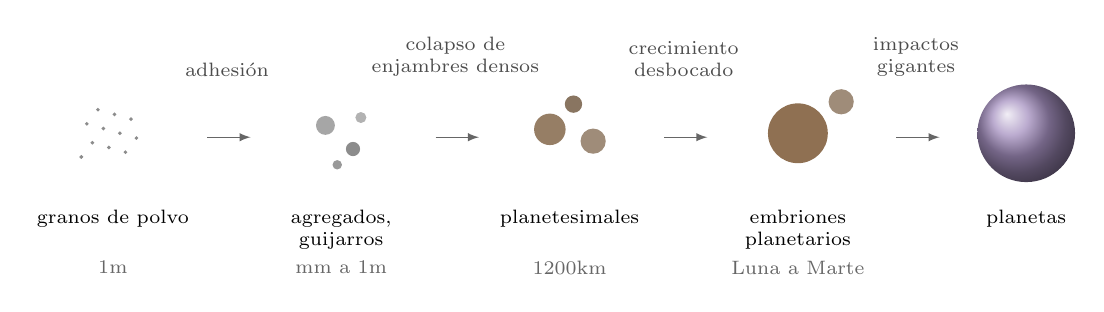
\begin{tikzpicture}[x=1cm, y=1cm, font=\scriptsize]
\foreach \x/\t/\s in {0/{granos de polvo}/{\qty{1}{\micro m}},
  2.9/{agregados,\\guijarros}/{mm a \qty{1}{m}},
  5.8/{planetesimales}/{\qtyrange{1}{200}{km}},
  8.7/{embriones\\planetarios}/{Luna a Marte},
  11.6/{planetas}/{} } {
  \node[align=center, anchor=north] at (\x,-0.9) {\t};
  \node[align=center, anchor=north, black!60] at (\x,-1.55) {\s};
}
\foreach \i in {0,...,11} {\fill[black!45] ({-0.4+0.07*mod(\i*7,11)},{-0.35+0.06*mod(\i*5,11)}) circle (0.025);}
\fill[black!35] (2.7,0.05) circle (0.12); \fill[black!45] (3.05,-0.25) circle (0.09);
\fill[black!40] (2.85,-0.45) circle (0.06); \fill[black!30] (3.15,0.15) circle (0.07);
\fill[brown!55!black!70] (5.55,0) circle (0.2); \fill[brown!50!black!60] (6.1,-0.15) circle (0.16);
\fill[brown!45!black!70] (5.85,0.32) circle (0.11);
\fill[brown!60!black!80] (8.7,-0.05) circle (0.38); \fill[brown!50!black!60] (9.25,0.35) circle (0.16);
\shade[ball color=blue!45!brown!60] (11.6,-0.05) circle (0.62);
\foreach \x in {1.2,4.1,7.0,9.95} {\draw[-latex, black!60] (\x,-0.1) -- +(0.55,0);}
\node[align=center, anchor=south, black!70] at (1.45,0.55) {adhesión};
\node[align=center, anchor=south, black!70] at (4.35,0.55) {colapso de\\enjambres densos};
\node[align=center, anchor=south, black!70] at (7.25,0.55) {crecimiento\\desbocado};
\node[align=center, anchor=south, black!70] at (10.2,0.55) {impactos\\gigantes};
\end{tikzpicture}

\par\smallskip{\small Del polvo a los planetas en la región de los planetas rocosos
(esquema, sin escala). Los granos se adhieren en agregados; los enjambres de guijarros colapsan
en \omterm{def:b2:planet-formation-meteorites:planetesimal}{planetesimales}; la gravedad hace que algunos \omterm{def:b2:planet-formation-meteorites:planetesimal}{planetesimales} crezcan desbocadamente hasta embriones, que
acaban fusionándose en planetas. Más allá de la \omterm{def:b2:planet-formation-meteorites:snow-line}{línea de nieve} los embriones crecieron más y pudieron
capturar gas. Tamaños según Chiang y Youdin (2010) y Lugaro y colaboradores (2018).}
% ledger: cy10:growth, lugaro:cai
\end{omfigure}

Los planetas conservaron poca memoria de esta historia: se fundieron, se mezclaron y
reelaboraron su materia. El registro está en los cuerpos que dejaron de crecer, los
asteroides, y en los fragmentos suyos que llegan a la Tierra.

\section{Los meteoritos}

\begin{definition}[Meteorito, caída de meteorito, hallazgo de meteorito]
\label{def:b2:planet-formation-meteorites:fall-find}
Un \emph{meteorito}\index{meteorito} es un objeto sólido natural procedente del espacio que
ha sobrevivido a su paso por la atmósfera y ha llegado al suelo. Una
\emph{caída de meteorito}\index{caída de meteorito} es un meteorito recogido después de que se
observara su llegada, por lo general como bola de fuego; un \emph{hallazgo de
meteorito}\index{hallazgo de meteorito} es un meteorito reconocido en el suelo sin que se haya
visto su caída.
\end{definition}

La Tierra barre mucho más polvo que piedras. Medido en la nieve de la
meseta antártica, unas \qty{5200}{t} de polvo extraterrestre llegan al
suelo cada año como micrometeoritos y esférulas fundidas, de unas
\qty{15000}{t} que entran en la atmósfera, la mayor parte desprendida por cometas y cerca de una
quinta parte por asteroides. Los \omterm{def:b2:planet-formation-meteorites:fall-find}{meteoritos}, las piedras y los hierros lo bastante grandes para
reconocerse uno a uno, son menos: el catálogo mundial contiene unos
\num{45000}, de los cuales solo \num{1107} son caídas.
% ledger: rojas21:flux, data:b4-meteorites

La distinción importa. Una caída se recoge en cuestión de días, antes de que la lluvia y el
oxígeno la hayan alterado, y todos los tipos de \omterm{def:b2:planet-formation-meteorites:fall-find}{meteorito} que caen se recogen
por igual; un hallazgo puede haber estado en el suelo miles de años, y su
probabilidad de ser encontrado depende de su aspecto y de dónde cayó. La mitad de todos
los hallazgos se han hecho en la Antártida (recuadro siguiente), donde la búsqueda es
sistemática. Las caídas son la muestra más fiel de lo que llega (figura siguiente):
más de cuatro de cada cinco son \omterm{def:b2:planet-formation-meteorites:chondrule}{condritas}, tres de cada cuatro \omterm{def:b2:planet-formation-meteorites:chondrule}{condritas} ordinarias.
% ledger: data:b4-meteorites

\begin{omfigure}
\begin{tikzpicture}
\begin{axis}[width=0.86\linewidth, height=6.3cm, ybar, bar width=7pt,
  xmin=0.4, xmax=9.6, ymin=0.1, ymax=200, ymode=log, log origin=infty,
  xtick={1,...,9}, xticklabels={ordinarias, carbonáceas, de enstatita, otras condritas,
    HED, otras acondritas, metálicos, metalorrocosos, sin clasificar},
  x tick label style={font=\scriptsize, rotate=30, anchor=north east, inner sep=1pt},
  tick label style={font=\scriptsize}, label style={font=\small},
  ylabel={proporción de la muestra (\%)}, legend pos=north east, xtick pos=bottom,
  legend style={font=\scriptsize, draw=black!30}, ymajorgrids, grid style={black!12}]
\addplot[fill=orange!70, draw=none] table[x=idx, y=falls_pct] {figdata/out/bachelor-2-meteorites-frac.dat};
\addlegendentry{caídas (\num{1107})}
\addplot[fill=blue!45, draw=none] table[x=idx, y=finds_pct] {figdata/out/bachelor-2-meteorites-frac.dat};
\addlegendentry{hallazgos (\num{44534})}
\end{axis}
\end{tikzpicture}

\par\smallskip{\small \omterm{def:b2:planet-formation-meteorites:fall-find}{Meteoritos} por clase, en porcentaje de las caídas y de los
hallazgos (escala logarítmica); HED: howarditas, eucritas y diogenitas. Datos: exportación de la NASA
de la Meteoritical Bulletin Database de The Meteoritical Society
(\num{45641} \omterm{def:b2:planet-formation-meteorites:fall-find}{meteoritos} válidos).}
% ledger: data:b4-meteorites
\end{omfigure}

\begin{inthefield}[La búsqueda de meteoritos en el hielo azul]
\begin{minipage}[t]{0.6\linewidth}\vspace{0pt}
La mayor parte del casquete antártico es nieve blanca, pero en cerca del
\qty{1}{\percent} de su superficie, donde las montañas bloquean el flujo del hielo,
se pierden unos \qty{5}{cm} de hielo al año y aflora hielo azul desnudo. Los \omterm{def:b2:planet-formation-meteorites:fall-find}{meteoritos}
que cayeron sobre la nieve aguas arriba, a lo largo de decenas de miles de años, quedan enterrados,
son transportados por el hielo y devueltos a la superficie donde este se consume:
el hielo azul es una trampa. Desde que empezó la recolección sistemática a mediados de la década de 1970,
los equipos han recuperado más de \num{30000} ejemplares de esos campos, y en
el catálogo la mitad de todos los hallazgos procede del sur de \ang{60}\,S. Los buscadores
recorren el hielo en líneas, a pie o en motos de nieve, y cada piedra encontrada se
recoge, por corriente que parezca, para que la colección no esté sesgada
hacia las llamativas. Cada hallazgo se fotografía donde yace, para registrar
su contexto, y recibe un número de campo; más tarde recibe su nombre oficial, un
código de tres letras del campo de hielo seguido del año de la campaña y de un
número de serie. En el laboratorio de conservación las piedras se fragmentan con
herramientas de acero inoxidable o se cortan en seco con una sierra de cinta; las \omterm{def:b2:planet-formation-meteorites:chondrule}{condritas carbonáceas},
que pueden contener compuestos orgánicos, tienen un armario propio desde 1978.
\end{minipage}\hfill
\begin{minipage}[t]{0.37\linewidth}\vspace{0pt}
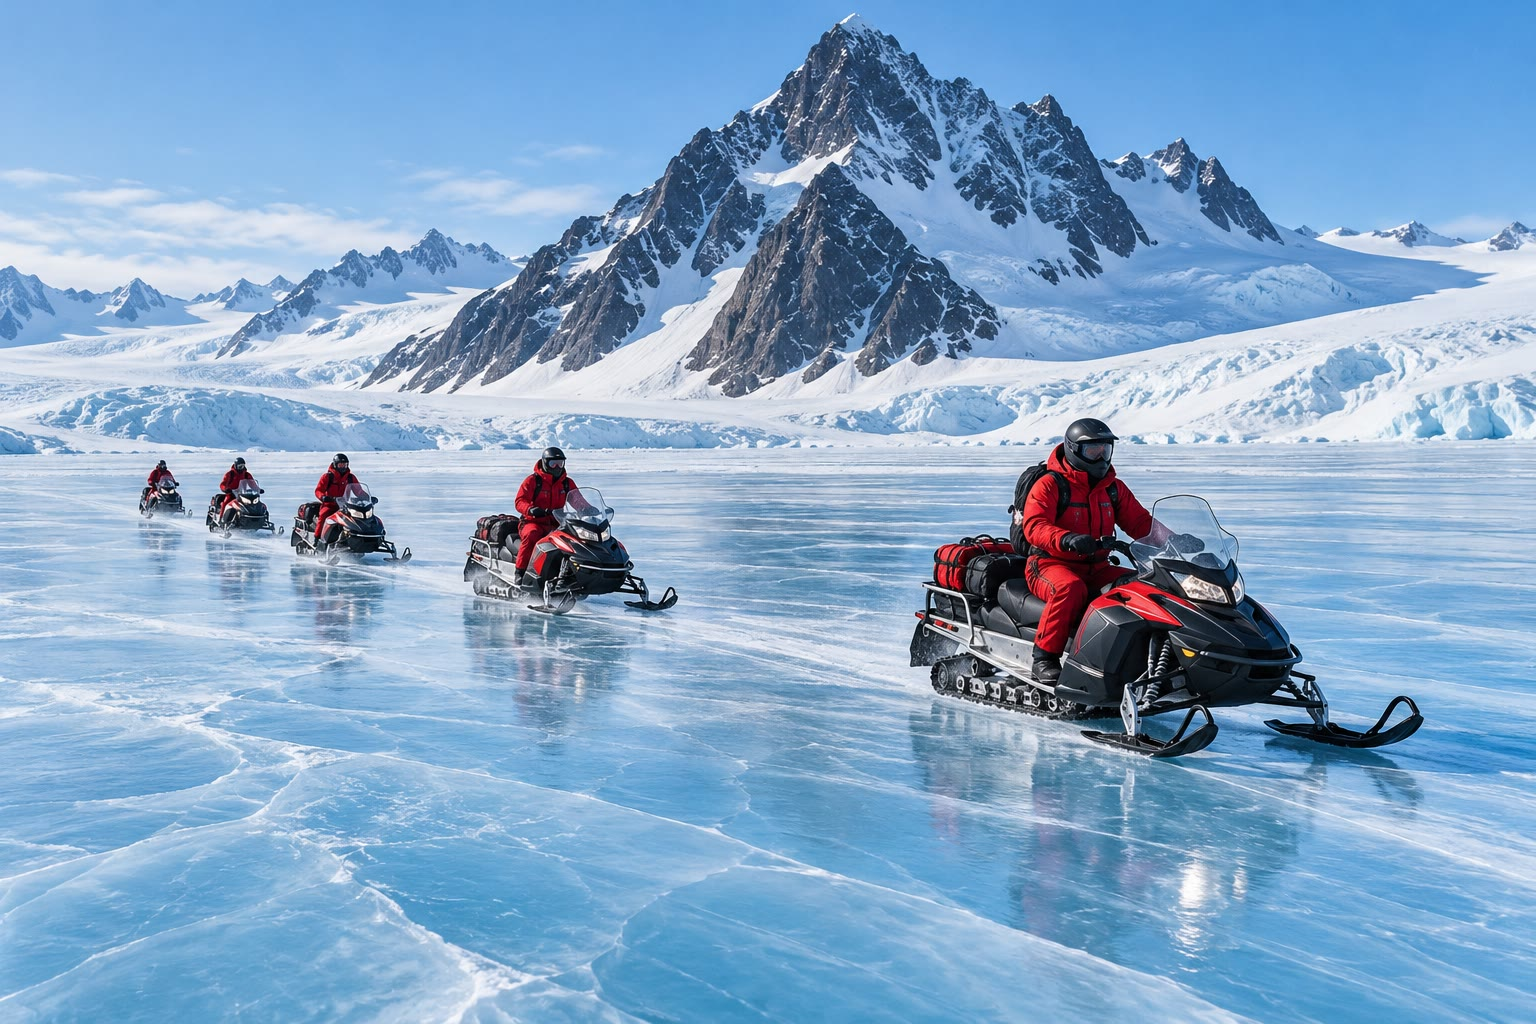
\includegraphics[width=\linewidth]{images/book4/ai/b2-blue-ice-search.jpg}

{\scriptsize Una línea de buscadores en motos de nieve cruza un campo de hielo azul al pie de
un pico rocoso (ilustración generada por IA).}
\end{minipage}
% ledger: folco06:blue-ice, data:b4-meteorites, nasa:antmet
\end{inthefield}

\subsection{Condritas}

\begin{definition}[Condrita, condrita carbonácea, cóndrulo, CAI]
\label{def:b2:planet-formation-meteorites:chondrule}
Una \emph{condrita}\index{condrita} es un \omterm{def:b2:planet-formation-meteorites:fall-find}{meteorito} rocoso que nunca se fundió
después de ensamblarse, y cuya composición, aparte de los elementos más volátiles,
es cercana a la del Sol. La mayor parte está formada por
\emph{cóndrulos}\index{cóndrulo}, gotitas redondeadas, de una décima de milímetro a
cerca de un centímetro de diámetro, de roca silicatada que solidificó a partir de un fundido, englobadas en
una matriz de grano fino con granos de metal hierro--níquel y de sulfuro de hierro. Algunas
condritas contienen \emph{inclusiones ricas en calcio y aluminio}\index{inclusión rica en calcio y aluminio}
(CAI), granos blancos irregulares de los minerales de calcio, aluminio
y titanio que son los primeros condensados de la nebulosa. Una
\emph{condrita carbonácea}\index{condrita carbonácea} es una condrita rica
en carbono, en minerales hidratados y en matriz, cuyo contenido en elementos volátiles
es el más cercano al del Sol.
\end{definition}

Los \omterm{def:b2:planet-formation-meteorites:chondrule}{cóndrulos} estuvieron fundidos solo unos minutos y se enfriaron en horas o
días: un calentamiento breve y local en la nebulosa, cuya causa aún se
desconoce, fundió grumos de polvo, que se solidificaron como gotitas antes de ser barridos
junto con polvo y metal hacia un \omterm{def:b2:planet-formation-meteorites:planetesimal}{planetesimal}. Ocupan hasta el \qty{90}{\percent} del volumen de los \omterm{def:b2:planet-formation-meteorites:fall-find}{meteoritos} más
primitivos. Las CAI suponen desde menos del \qty{1}{\percent} de las
\omterm{def:b2:planet-formation-meteorites:chondrule}{condritas} ordinarias hasta más del \qty{10}{\percent} de algunas carbonáceas, y
se formaron en un intervalo de unos cien mil años.
% ledger: gail:meteorites, cy10:growth, cy10:chondrules, gail:chondrite-table, lugaro:cai

\begin{omfigure}
\begin{minipage}[c]{0.5\linewidth}
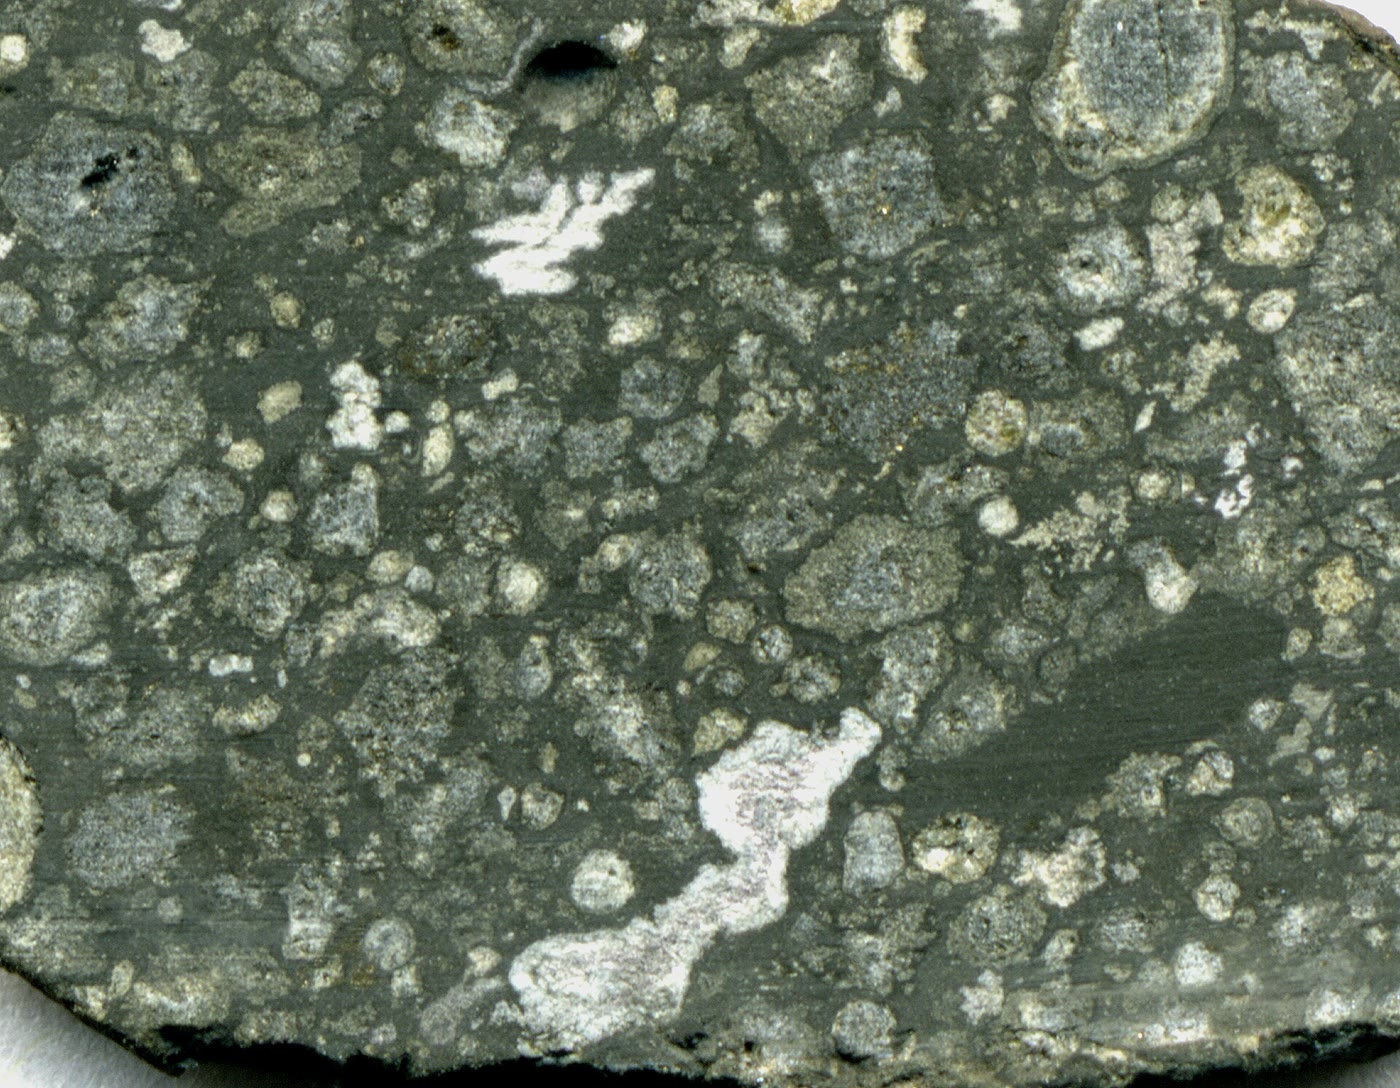
\includegraphics[width=\linewidth]{images/book4/b2-allende-chondrite.jpg}
\end{minipage}\hfill
\begin{minipage}[c]{0.46\linewidth}
{\small Cara cortada de la \omterm{def:b2:planet-formation-meteorites:chondrule}{condrita carbonácea} de Allende (clase CV3), que cayó en
el norte de México en 1969: se recogieron unas dos toneladas. Los granos grises redondeados son
\omterm{def:b2:planet-formation-meteorites:chondrule}{cóndrulos}; las manchas blancas irregulares son CAI; el cemento oscuro es la matriz. El
campo mide unos pocos centímetros. James St.\ John, CC BY 2.0.}
\end{minipage}
% ledger: data:b4-meteorites, gail:chondrite-table
\end{omfigure}

Las \omterm{def:b2:planet-formation-meteorites:chondrule}{condritas} se dividen en grupos que difieren en el tamaño y la abundancia de sus
\omterm{def:b2:planet-formation-meteorites:chondrule}{cóndrulos}, su contenido en metal, el contenido en hierro de su olivino y la
proporción de su matriz (tabla siguiente). Las \omterm{def:b2:planet-formation-meteorites:chondrule}{condritas} ordinarias H, L y LL
tienen contenidos altos, bajos y muy bajos de metal y de hierro total (razones atómicas
Fe/Si de \num{0.80}, \num{0.59} y \num{0.53}).
% ledger: gail:chondrite-table

\begin{table}[h]
\centering
\small
\begin{tabular}{lcccccc}
\hline
 & H & L & LL & CI & CM & CV\\
\hline
\omterm{def:b2:planet-formation-meteorites:chondrule}{cóndrulos} (vol.\ \%) & 60--80 & 60--80 & 60--80 & $\ll 1$ & 20 & 45\\
diámetro medio de los \omterm{def:b2:planet-formation-meteorites:chondrule}{cóndrulos} (mm) & 0.3 & 0.7 & 0.9 & --- & 0.3 & 1.0\\
CAI (vol.\ \%) & 0.1--1 & 0.1--1 & 0.1--1 & $\ll 1$ & 5 & 10\\
matriz (vol.\ \%) & 10--15 & 10--15 & 10--15 & $> 99$ & 70 & 40\\
metal hierro--níquel (vol.\ \%) & 10 & 5 & 2 & 0 & 0.1 & 0--5\\
fayalita en el olivino (mol \%) & 16--20 & 23--26 & 27--32 & & & \\
\omterm{def:b2:planet-formation-meteorites:type}{tipos petrológicos} & 3--6 & 3--6 & 3--6 & 1 & 2 & 3\\
temperatura máxima (K) & 1220 & 1220 & 1220 & 430 & 670 & 870\\
\hline
\end{tabular}
\caption{Propiedades de las \omterm{def:b2:planet-formation-meteorites:chondrule}{condritas} ordinarias (H, L, LL) y de tres grupos de \omterm{def:b2:planet-formation-meteorites:chondrule}{condritas
carbonáceas}. Fayalita: el término extremo férrico del olivino. Datos: Gail y colaboradores (2014).}
\label{tab:b2:planet-formation-meteorites:chondrites}
% ledger: gail:chondrite-table
\end{table}

\begin{definition}[Tipo petrológico]\label{def:b2:planet-formation-meteorites:type}
El \emph{tipo petrológico}\index{tipo petrológico} de una \omterm{def:b2:planet-formation-meteorites:chondrule}{condrita} es un número
de 1 a 6 que registra lo que le ocurrió en su cuerpo progenitor: el tipo 3 es el
menos alterado; los tipos 4 a 6 están cada vez más calentados, con los \omterm{def:b2:planet-formation-meteorites:chondrule}{cóndrulos} difuminados
y los minerales recristalizados y de composición uniforme; los tipos 2 y 1 están
cada vez más alterados por agua líquida, que transformó sus minerales en arcillas.
\end{definition}

La última fila de la tabla da las temperaturas máximas alcanzadas por cada grupo:
hasta unos \qty{1220}{K} para las \omterm{def:b2:planet-formation-meteorites:chondrule}{condritas} ordinarias más calentadas, nunca más
de \qty{430}{K} para las \omterm{def:b2:planet-formation-meteorites:chondrule}{condritas} CI, empapadas de agua pero nunca calientes. El
calentamiento, como muestra la última sección, vino del interior de los cuerpos progenitores.
% ledger: gail:chondrite-table

\subsection{Acondritas y meteoritos metálicos}

\begin{definition}[Acondrita, meteorito metálico, meteorito metalorrocoso]
\label{def:b2:planet-formation-meteorites:classes}
Una \emph{acondrita}\index{acondrita} es un \omterm{def:b2:planet-formation-meteorites:fall-find}{meteorito} rocoso que cristalizó
a partir de un fundido o recristalizó a alta temperatura en un cuerpo que se fundió, y
por eso no tiene \omterm{def:b2:planet-formation-meteorites:chondrule}{cóndrulos}. Un \emph{meteorito metálico}\index{meteorito metálico} está formado
sobre todo por metal hierro--níquel. Un \emph{meteorito
metalorrocoso}\index{meteorito metalorrocoso} está formado por metal y silicato en cantidades
aproximadamente iguales.
\end{definition}

Son los fragmentos de cuerpos que se fundieron y se diferenciaron: las \omterm{def:b2:planet-formation-meteorites:classes}{acondritas} son sus
cortezas y sus mantos, los \omterm{def:b2:planet-formation-meteorites:classes}{meteoritos metálicos} sus núcleos de metal, y los metalorrocosos proceden del lugar donde
se encontraban el metal y el silicato. La mayor familia de \omterm{def:b2:planet-formation-meteorites:classes}{acondritas}, las howarditas,
eucritas y diogenitas (HED), basaltos y rocas ricas en piroxeno, supone el
\qty{5.5}{\percent} de todas las caídas. Su origen se rastreó, por su espectro y
su órbita, hasta el asteroide Vesta, de unos \qty{525}{km} de diámetro, y la sonda
Dawn, que llegó a Vesta en 2011, lo confirmó: la química
y la mineralogía de la superficie de Vesta coinciden con las de los \omterm{def:b2:planet-formation-meteorites:fall-find}{meteoritos} HED, una cuenca
de \qty{500}{km} de anchura cerca de su polo sur muestra de dónde se arrancaron los fragmentos,
y su campo de gravedad indica un núcleo de hierro de unos \qty{225}{km} de diámetro.
Vesta se fundió, casi o por completo, al principio de su historia. Otras \omterm{def:b2:planet-formation-meteorites:classes}{acondritas} proceden
de la Luna y de Marte. Los \omterm{def:b2:planet-formation-meteorites:fall-find}{meteoritos} de las colecciones parecen proceder
de un centenar de cuerpos progenitores distintos.
% ledger: data:b4-meteorites, nasa:vesta-dawn, gail:meteorites

Los \omterm{def:b2:planet-formation-meteorites:classes}{meteoritos metálicos} guardan el registro de cómo se enfriaron sus núcleos. Una cara cortada y
atacada con ácido muestra un entramado de láminas (figura siguiente): a alta
temperatura el metal es una sola aleación de hierro y níquel; al enfriarse lentamente, una
aleación pobre en níquel crece en láminas a lo largo de los planos del cristal original,
y cuanto más lento es el enfriamiento, más anchas son las láminas. Medidas en muchos \omterm{def:b2:planet-formation-meteorites:classes}{meteoritos metálicos}, las
anchuras de las láminas dan las velocidades de enfriamiento de los núcleos de los que proceden.
% ledger: gail:meteorites

\begin{omfigure}
\begin{minipage}[c]{0.5\linewidth}
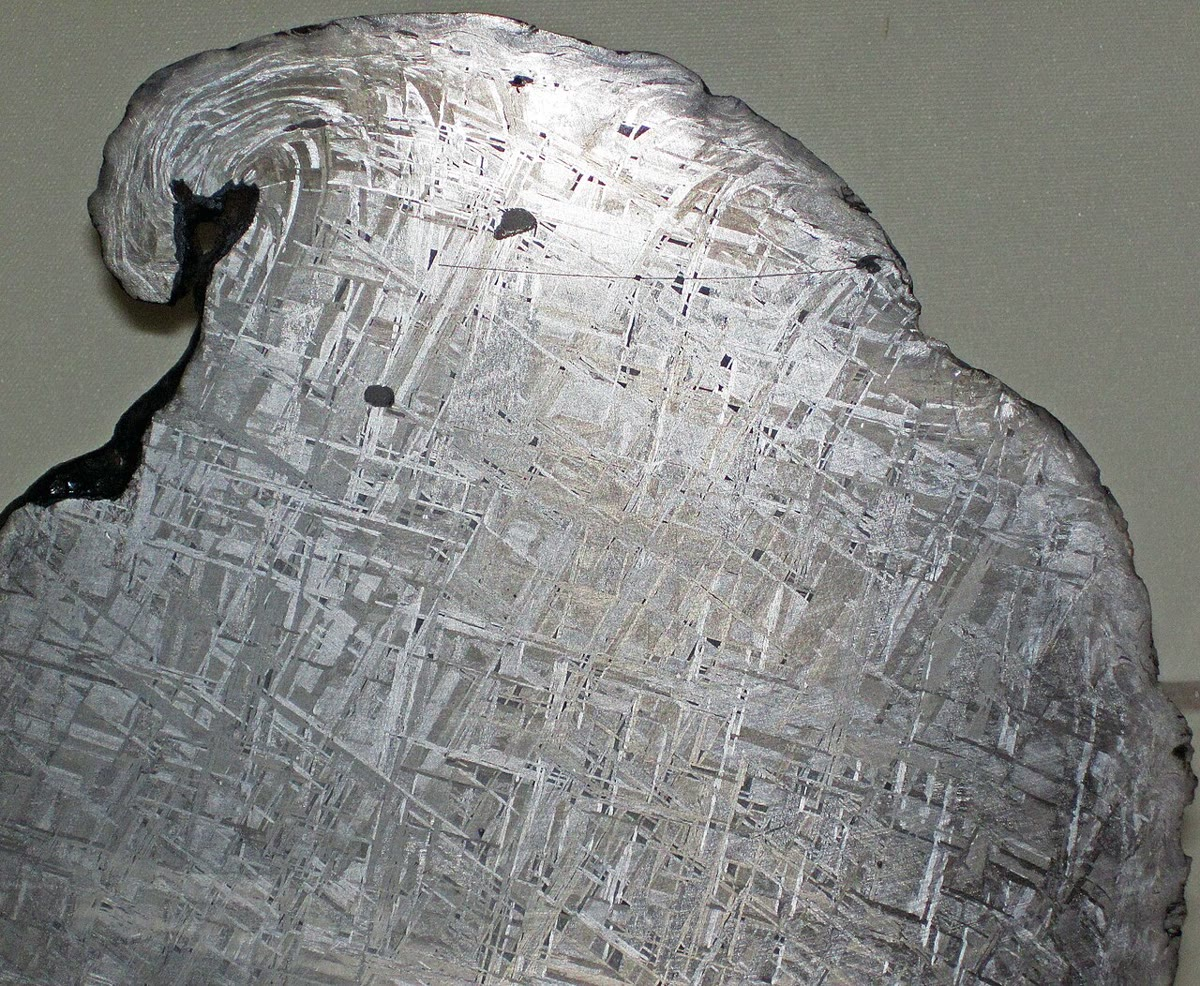
\includegraphics[width=\linewidth]{images/book4/b2-gibeon-widmanstatten.jpg}
\end{minipage}\hfill
\begin{minipage}[c]{0.46\linewidth}
{\small Cara cortada, pulida y atacada con ácido de un fragmento del \omterm{def:b2:planet-formation-meteorites:classes}{meteorito metálico} Gibeon,
hallado en Namibia: el entramado de láminas de aleación hierro--níquel (las figuras de
Widmanstätten) creció al enfriarse lentamente el núcleo metálico de su cuerpo progenitor. James St.\ John,
CC BY 2.0.}
\end{minipage}
% ledger: data:b4-meteorites
\end{omfigure}

\section{La datación del sistema solar}

La edad del sistema solar es la edad de sus sólidos más antiguos. Las isócronas
uranio--plomo de las CAI, construidas como en el volumen de primer año, dan \qtyrange{4567}{4568}{\Ma};
las CAI se formaron en un intervalo de unos \qty{0.1}{Myr}, un tiempo lo bastante corto
para tomar su edad como el nacimiento del Sol. Los acontecimientos de los
pocos millones de años siguientes, la formación de los \omterm{def:b2:planet-formation-meteorites:chondrule}{cóndrulos} y el ensamblaje y la
fusión de los primeros cuerpos, se datan mejor con respecto a las CAI, con relojes
que corrían deprisa y se pararon pronto.
% ledger: lugaro:cai

\begin{definition}[Radionúclido de vida corta]
\label{def:b2:planet-formation-meteorites:slr}
Un \emph{radionúclido de vida corta}\index{radionúclido de vida corta} es un
nucleido radiactivo con un periodo de semidesintegración de aproximadamente \num{0.1} a \qty{100}{Myr},
presente cuando se formó el sistema solar y hoy extinto, cuya presencia pasada
se manifiesta por un exceso de su hijo en minerales que eran ricos en su
elemento.
\end{definition}

El más conocido es el aluminio-26, que se desintegra en magnesio-26 con un periodo de semidesintegración de
\qty{0.717}{Myr} (una vida media de \qty{1.035}{Myr}). Cuando se formaron las CAI, uno de
cada \num{19000} átomos de aluminio era aluminio-26: la razón
$\ce{^{26}Al}/\ce{^{27}Al}$ era $(5.23 \pm 0.13)\times10^{-5}$, el valor
\emph{canónico}. Otros nucleidos de vida corta cubren intervalos más largos (tabla
siguiente).
% ledger: lugaro:al26, lugaro:slr-table

\begin{table}[h]
\centering
\small
\begin{tabular}{lllcc}
\hline
nucleido & hijo & referencia & periodo (Myr) & razón inicial\\
\hline
\ce{^{26}Al} & \ce{^{26}Mg} & \ce{^{27}Al} & 0.717 & $5.23\times10^{-5}$\\
\ce{^{60}Fe} & \ce{^{60}Ni} & \ce{^{56}Fe} & 2.62 & $1.0\times10^{-8}$\\
\ce{^{53}Mn} & \ce{^{53}Cr} & \ce{^{55}Mn} & 3.74 & $7\times10^{-6}$\\
\ce{^{107}Pd} & \ce{^{107}Ag} & \ce{^{108}Pd} & 6.5 & $6.6\times10^{-5}$\\
\ce{^{182}Hf} & \ce{^{182}W} & \ce{^{180}Hf} & 8.90 & $1.02\times10^{-4}$\\
\ce{^{129}I} & \ce{^{129}Xe} & \ce{^{127}I} & 15.7 & $1.28\times10^{-4}$\\
\hline
\end{tabular}
\caption{Algunos \omterm{def:b2:planet-formation-meteorites:slr}{radionúclidos de vida corta} del sistema solar primitivo, su hijo
estable, el isótopo estable del mismo elemento usado como referencia, su
periodo de semidesintegración y su razón respecto a la referencia cuando se formaron las CAI. Datos: Lugaro y
colaboradores (2018).}
\label{tab:b2:planet-formation-meteorites:slr}
% ledger: lugaro:al26, lugaro:slr-table
\end{table}

\begin{proposition}[Edad relativa a partir de un nucleido extinto]
\label{prop:b2:planet-formation-meteorites:relative-age}
Si la razón de un nucleido de vida corta a su isótopo de referencia valía $R_0$
en todas partes cuando se formaron las CAI, y se halla que valía $R$ en un objeto cuando
este se formó, el objeto se formó
\[
  \Delta t = \tau \ln\frac{R_0}{R}
\]
después de las CAI, donde $\tau$ es la vida media del nucleido. Un error
$\delta R$ en $R$ da el error $\tau\,\delta R/R$ en $\Delta t$.
\end{proposition}

\begin{proof}
El isótopo de referencia es estable, de modo que la razón decrece como el propio
nucleido radiactivo: $R = R_0 e^{-\Delta t/\tau}$. Tomando logaritmos,
$\Delta t = \tau\ln(R_0/R)$. Derivando, $\mathrm d(\Delta t) =
-\tau\,\mathrm dR/R$.
\end{proof}

Un error relativo del \qty{10}{\percent} en la razón cuesta así
\qty{0.1}{Myr} con el aluminio-26, pero \qty{0.54}{Myr} con el manganeso-53 y
\qty{1.3}{Myr} con el hafnio-182: cada reloj solo es preciso a lo largo de unas pocas de sus
propias vidas medias, y el reloj adecuado depende del acontecimiento. La razón $R$ de un
objeto se lee en sus minerales.
% ledger: lugaro:al26, lugaro:slr-table

\begin{proposition}[Isócrona aluminio--magnesio]
\label{prop:b2:planet-formation-meteorites:al-mg}
Supóngase que varios minerales de un objeto se forman juntos en el tiempo $\Delta t$ con la
misma composición isotópica del magnesio, $(\ce{^{26}Mg}/\ce{^{24}Mg})_0$, pero
con razones $\ce{^{27}Al}/\ce{^{24}Mg}$ distintas, y permanecen cerrados desde entonces. Hoy se
alinean en la recta
\[
  \frac{\ce{^{26}Mg}}{\ce{^{24}Mg}}
  = \left(\frac{\ce{^{26}Mg}}{\ce{^{24}Mg}}\right)_0
  + R\,\frac{\ce{^{27}Al}}{\ce{^{24}Mg}},
\]
cuya pendiente es la razón $R = \ce{^{26}Al}/\ce{^{27}Al}$ del objeto cuando se
formó.
\end{proposition}

\begin{proof}
Cada átomo de aluminio-26 presente en la formación se ha convertido desde entonces en un
átomo de magnesio-26, de modo que un mineral ha ganado
$\ce{^{26}Al}_{\text{inicial}} = R\,\ce{^{27}Al}$ átomos de magnesio-26, ya que el aluminio-27
es estable. Dividiendo por el número de átomos de magnesio-24, que no cambia,
se obtiene la recta.
\end{proof}

Los minerales ricos en aluminio y pobres en magnesio, como la plagioclasa, muestran grandes excesos
de magnesio-26; el olivino, casi libre de aluminio, no muestra ninguno. Así se construyó
la secuencia temporal del sistema solar primitivo: primero las CAI; los \omterm{def:b2:planet-formation-meteorites:chondrule}{cóndrulos} a lo largo de
los pocos millones de años siguientes, con unos datos de los \omterm{def:b2:planet-formation-meteorites:chondrule}{cóndrulos} que fijan la
duración del disco de gas en menos de cinco millones de años; los cuerpos progenitores de
las \omterm{def:b2:planet-formation-meteorites:chondrule}{condritas} se ensamblaron después de sus \omterm{def:b2:planet-formation-meteorites:chondrule}{cóndrulos} más jóvenes. Las diogenitas,
rocas del manto de Vesta, empezaron a cristalizar en el primer millón de años tras
las CAI, y el núcleo de Vesta se formó en los primeros uno a
cuatro millones de años: los \omterm{def:b2:planet-formation-meteorites:classes}{meteoritos metálicos} y las \omterm{def:b2:planet-formation-meteorites:classes}{acondritas} son más antiguos que muchas
\omterm{def:b2:planet-formation-meteorites:chondrule}{condritas}.
% ledger: lugaro:cai, gail:vesta, gail:meteorites

\section{El calor del aluminio-26 y la primera fusión}

¿De dónde vino el calor que fundió Vesta y metamorfizó las \omterm{def:b2:planet-formation-meteorites:chondrule}{condritas}
ordinarias? Los modelos y los \omterm{def:b2:planet-formation-meteorites:fall-find}{meteoritos} coinciden en que en los cuerpos más antiguos
la fuente dominante fue la desintegración del aluminio-26. En una roca de composición condrítica aportaba, al principio,
\qty{5}{MJ} por kilogramo listos para liberarse en unos pocos millones de años:
suficiente para calentar la roca miles de kelvin, si el calor no podía escapar.
% ledger: lugaro:heat, lugaro:melting

\begin{proposition}[Calentamiento de un planetesimal por el aluminio-26]
\label{prop:b2:planet-formation-meteorites:heating}
Una roca que recibe la potencia radiactiva $H_0 e^{-t/\tau}$ por kilogramo, de
capacidad calorífica específica $c$ y que no pierde calor, se calienta tras su acreción en
el tiempo $t_a$ según
\[
  T(t) = T_0 + \frac{H_0\tau}{c}\left(e^{-t_a/\tau} - e^{-t/\tau}\right),
\]
y tiende a la temperatura máxima
$T_{\max} = T_0 + (H_0\tau/c)\,e^{-t_a/\tau}$. Una temperatura crítica
$T_c > T_0$ solo se alcanza si el cuerpo se acretó antes de
\[
  t_a^* = \tau\ln\frac{H_0\tau}{c\,(T_c - T_0)}.
\]
\end{proposition}

\begin{proof}
Sin pérdidas, $c\,\mathrm dT/\mathrm dt = H_0 e^{-t/\tau}$. Integrando desde
$t_a$, donde $T = T_0$, se obtiene
$c\,(T - T_0) = H_0\tau\,(e^{-t_a/\tau} - e^{-t/\tau})$, que tiende a
$H_0\tau e^{-t_a/\tau}$ cuando $t \to \infty$. Imponiendo $T_{\max} = T_c$ y despejando
$t_a$ se obtiene $t_a^*$; para una acreción más temprana el máximo es más alto.
\end{proof}

Un modelo del cuerpo progenitor de las \omterm{def:b2:planet-formation-meteorites:chondrule}{condritas} ordinarias usa
$H_0 = \qty{1.9e-7}{W.kg^{-1}}$, $c = \qty{837}{J.kg^{-1}.K^{-1}}$ y
$T_0 = \qty{250}{K}$. Entonces $H_0\tau/c$ vale unos \qty{7400}{K}. Importan tres
temperaturas: hacia \qty{750}{K} la roca porosa empieza a sinterizarse en una
roca compacta; hacia \qty{1200}{K} el metal y el sulfuro de hierro empiezan a fundirse
juntos; hacia \qty{1700}{K} se funden los últimos silicatos. Un cuerpo que se acretó
antes de \qty{1.7}{Myr} se fundió por completo; antes de \qty{2.1}{Myr} su metal y su sulfuro
se fundieron y pudieron hundirse para formar un núcleo; hasta unos \qty{2.8}{Myr} quedó al menos
sinterizado y metamorfizado; los cuerpos posteriores siguieron fríos (figura siguiente).
% ledger: gail:params, gail:temps, lugaro:al26

\begin{omfigure}
\begin{tikzpicture}
\begin{axis}[omrecord, name=left, width=0.45\linewidth, height=6.0cm,
  xmin=0, xmax=8, ymin=0, ymax=2300,
  xlabel={tiempo tras las CAI (Myr)}, ylabel={temperatura (K)},
  tick label style={font=\scriptsize}, label style={font=\small}]
\addplot[black!45, densely dashed, domain=0:8, samples=2] {750};
\addplot[black!45, densely dashed, domain=0:8, samples=2] {1200};
\addplot[black!45, densely dashed, domain=0:8, samples=2] {1700};
\addplot[thick, red!75!black] table[x=t_Myr, y=T_K] {figdata/out/bachelor-2-al26-ta15.dat};
\addplot[thick, orange!80!black] table[x=t_Myr, y=T_K] {figdata/out/bachelor-2-al26-ta20.dat};
\addplot[thick, teal!70!black] table[x=t_Myr, y=T_K] {figdata/out/bachelor-2-al26-ta25.dat};
\addplot[thick, blue!70!black] table[x=t_Myr, y=T_K] {figdata/out/bachelor-2-al26-ta30.dat};
\node[font=\tiny, red!75!black, anchor=south east] at (axis cs:7.9,1995) {$t_a = \qty{1.5}{Myr}$};
\node[font=\tiny, orange!80!black, anchor=south east] at (axis cs:7.9,1325) {2};
\node[font=\tiny, teal!70!black, anchor=south east] at (axis cs:7.9,915) {2.5};
\node[font=\tiny, blue!70!black, anchor=north east] at (axis cs:7.9,650) {3};
\node[font=\tiny, black!60, anchor=south west] at (axis cs:0.1,1700) {silicatos fundidos};
\node[font=\tiny, black!60, anchor=south west] at (axis cs:0.1,1200) {fusión de Fe--FeS};
\node[font=\tiny, black!60, anchor=south west] at (axis cs:0.1,750) {sinterización};
\end{axis}
\begin{axis}[omrecord, at={(left.east)}, anchor=west, xshift=2.1cm, width=0.45\linewidth,
  height=6.0cm, xmin=0, xmax=4, ymin=0, ymax=8000,
  xlabel={momento de acreción $t_a$ (Myr)}, ylabel={temperatura máxima (K)},
  tick label style={font=\scriptsize}, label style={font=\small},
  scaled y ticks=false, yticklabel style={/pgf/number format/1000 sep={\,}}]
\addplot[black!45, densely dashed, domain=0:4, samples=2] {750};
\addplot[black!45, densely dashed, domain=0:4, samples=2] {1200};
\addplot[black!45, densely dashed, domain=0:4, samples=2] {1700};
\addplot[thick, black] table[x=ta_Myr, y=Tpeak_K] {figdata/out/bachelor-2-al26-peak.dat};
\draw[black!60] (axis cs:1.69,0) -- (axis cs:1.69,1700);
\draw[black!60] (axis cs:2.13,0) -- (axis cs:2.13,1200);
\node[font=\tiny, black!70, anchor=south] at (axis cs:2.0,4500) {\qty{1.7}{Myr}};
\draw[black!50, -latex] (axis cs:2.0,4450) -- (axis cs:1.71,1800);
\node[font=\tiny, black!70, anchor=south] at (axis cs:2.9,3300) {\qty{2.1}{Myr}};
\draw[black!50, -latex] (axis cs:2.9,3250) -- (axis cs:2.16,1300);
\end{axis}
\end{tikzpicture}

\par\smallskip{\small Calentamiento por el aluminio-26 del interior de un cuerpo condrítico sin
pérdidas de calor (la proposición anterior; $H_0 = \qty{1.9e-7}{W.kg^{-1}}$,
$c = \qty{837}{J.kg^{-1}.K^{-1}}$, $T_0 = \qty{250}{K}$, $\tau = \qty{1.035}{Myr}$).
Izquierda: temperatura frente al tiempo para cuerpos acretados 1.5, 2, 2.5 y \qty{3}{Myr}
después de las CAI. Derecha: temperatura máxima frente al momento de acreción; los cuerpos acretados
antes de \qty{1.7}{Myr} se fundieron, y antes de \qty{2.1}{Myr} se fundieron su metal y su sulfuro.
Los cuerpos reales gastan parte del calor en la fusión, lo que limita la temperatura, y pierden
calor cerca de su superficie. Valores del modelo: Gail y colaboradores (2014).}
% ledger: gail:params, gail:temps, lugaro:al26
\end{omfigure}

La proposición ignora las pérdidas de calor, lo que solo es válido en lo profundo de un cuerpo grande.
El calor se difunde a lo largo de la distancia $\sqrt{\kappa t}$ en el tiempo $t$, donde
$\kappa$ es la difusividad térmica de la roca: con los valores del modelo,
unos \qty{5}{km} en una vida media del aluminio-26 (\cref{exo:b2:planet-formation-meteorites:12}). Los cuerpos mucho
más pequeños que esto pierden su calor tan deprisa como lo producen; los modelos detallados muestran
que los cuerpos de más de \qtyrange{10}{20}{km} de diámetro podían fundirse.
% ledger: gail:params, lugaro:melting

\begin{definition}[Diferenciación planetaria]
\label{def:b2:planet-formation-meteorites:differentiation}
La \emph{diferenciación planetaria}\index{diferenciación planetaria} es la
separación de un cuerpo, total o parcialmente fundido, en capas de distinta
composición y densidad: un núcleo de metal, un manto de silicatos y una corteza formada por
los últimos fundidos.
\end{definition}

Los \omterm{def:b2:planet-formation-meteorites:fall-find}{meteoritos} registran así dos tipos de cuerpos primitivos. Los que se formaron en
los dos primeros millones de años aproximadamente tenían aluminio-26 suficiente para fundirse y
diferenciarse: sus núcleos son los \omterm{def:b2:planet-formation-meteorites:classes}{meteoritos metálicos}, sus cortezas y mantos
las \omterm{def:b2:planet-formation-meteorites:classes}{acondritas}, y Vesta es la superviviente. Los que se formaron más tarde siguieron siendo
\omterm{def:b2:planet-formation-meteorites:chondrule}{condritas}, calentadas desde dentro en un grado fijado por su fecha de nacimiento y por
la profundidad de cada fragmento: los más profundos llegaron al tipo 6, los más superficiales se quedaron en el
tipo 3. La propia Tierra, construida con embriones y \omterm{def:b2:planet-formation-meteorites:planetesimal}{planetesimales} de ambos tipos y
golpeada por impactos gigantes, se diferenció en núcleo, manto y corteza.
% ledger: gail:meteorites, gail:vesta, gail:temps

\section{Ejercicios}

\begin{exercise}[$\star$]\label{exo:b2:planet-formation-meteorites:1}
En la \omterm{def:b2:planet-formation-meteorites:nebula}{nebulosa solar} de masa mínima, calcúlese la densidad superficial del gas a
\qty{1}{au} y a \qty{5.2}{au}, y la densidad superficial de los sólidos a
\qty{1}{au} (solo roca, $Z_{\mathrm{rel}} = 0.33$) y a \qty{5.2}{au} (todos los hielos
condensados, $Z_{\mathrm{rel}} = 1$). ¿Cuántas veces más pesado que los sólidos es el
gas a \qty{5.2}{au}?
% ledger: cy10:mmsn
\end{exercise}

\begin{exercise}[$\star$]\label{exo:b2:planet-formation-meteorites:2}
Con la figura de las \omterm{def:b2:planet-formation-meteorites:condensation}{temperaturas de condensación}, ordénense el aluminio, el sodio,
el magnesio, el hierro, el azufre y el oxígeno (como hielo de agua) del primero en condensar al
último, y dese el grupo de volatilidad de cada uno. ¿Cuáles cabría esperar
enriquecidos en las CAI, y cuáles empobrecidos en la Tierra respecto al Sol?
% ledger: lodders:tc-table, lodders:groups
\end{exercise}

\begin{exercise}[$\star$]\label{exo:b2:planet-formation-meteorites:3}
El catálogo recoge \num{1107} caídas, de las cuales 856 son \omterm{def:b2:planet-formation-meteorites:chondrule}{condritas} ordinarias y
49 \omterm{def:b2:planet-formation-meteorites:classes}{meteoritos metálicos}, y \num{44534} hallazgos, de los cuales \num{38647} son \omterm{def:b2:planet-formation-meteorites:chondrule}{condritas} ordinarias,
\num{1020} metálicos y \num{22096} proceden del sur de \ang{60}\,S. Calcúlese la
proporción de \omterm{def:b2:planet-formation-meteorites:chondrule}{condritas} ordinarias y de \omterm{def:b2:planet-formation-meteorites:classes}{meteoritos metálicos} entre las caídas y entre los hallazgos,
y la proporción de hallazgos antárticos. ¿Qué muestra se usaría para estimar las
proporciones en que llegan las clases a la Tierra, y por qué?
% ledger: data:b4-meteorites
\end{exercise}

\begin{exercise}[$\star$]\label{exo:b2:planet-formation-meteorites:4}
Los minerales de un objeto dan la razón inicial
$\ce{^{26}Al}/\ce{^{27}Al} = \num{1.0e-5}$. ¿Cuánto tiempo después de las CAI se formó?
Tómense $R_0 = \num{5.23e-5}$ y una vida media de \qty{1.035}{Myr}.
% ledger: lugaro:al26
\end{exercise}

\begin{exercise}[$\star\star$]\label{exo:b2:planet-formation-meteorites:5}
Con la \cref{prop:b2:planet-formation-meteorites:disc-mass} y
$\Sigma_1 = \qty{2.2e4}{kg.m^{-2}}$ a \qty{1}{au} (\qty{1}{au} $=
\qty{1.496e11}{m}$, $M_\odot = \qty{1.989e30}{kg}$), calcúlese la masa de la
nebulosa de masa mínima dentro de \qty{30}{au} y dentro de \qty{100}{au}, en masas
solares. Compárese con los discos observados, \numrange{0.001}{0.1} masas solares.
% ledger: cy10:mmsn
\end{exercise}

\begin{exercise}[$\star\star$]\label{exo:b2:planet-formation-meteorites:6}
En el disco pasivo $T = \qty{120}{K}\,(r/\qty{1}{au})^{-3/7}$, hállese dónde se vuelven estables el hielo
de agua (\qty{182}{K}) y el hielo de metano (\qty{41}{K}). Un grano bajo luz solar
directa alcanza \qty{182}{K} a \qty{2.3}{au}. ¿Por qué difieren las dos estimaciones de la
\omterm{def:b2:planet-formation-meteorites:snow-line}{línea de nieve}, y cuál se aplica a los cuerpos que construyeron los planetas?
% ledger: cy10:passive, lodders:phases
\end{exercise}

\begin{exercise}[$\star\star$]\label{exo:b2:planet-formation-meteorites:7}
Calcúlese la masa de aislamiento, con $b = 5$, de un embrión a \qty{1}{au} en la
nebulosa de masa mínima ($\Sigma_p = \qty{10.9}{g.cm^{-2}}$), y a \qty{5.2}{au}
más allá de la \omterm{def:b2:planet-formation-meteorites:snow-line}{línea de nieve} ($\Sigma_p = \qty{2.78}{g.cm^{-2}}$), en masas terrestres
($M_\oplus = \qty{5.972e24}{kg}$, $M_\odot = \qty{1.989e30}{kg}$). ¿En cuánto se
convierte a \qty{5.2}{au} en un disco con \num{3.5} veces más sólidos?
% ledger: cy10:isolation, cy10:mmsn, earth:mass
\end{exercise}

\begin{exercise}[$\star\star$]\label{exo:b2:planet-formation-meteorites:8}
Una roca de composición CI contenía \num{1.01e16} átomos de aluminio-26 por gramo cuando
se formaron las CAI, y cada desintegración deja \qty{5.00e-13}{J} de calor. Calcúlese el
calor liberado por kilogramo a lo largo de toda la desintegración, y el aumento de temperatura que
produciría con $c = \qty{837}{J.kg^{-1}.K^{-1}}$ y sin pérdidas. ¿Cuántas veces
supera al calor necesario para calentar la roca de \num{250} a
\qty{1700}{K}?
% ledger: lugaro:heat, gail:params
\end{exercise}

\begin{exercise}[$\star\star$]\label{exo:b2:planet-formation-meteorites:9}
A lo largo de toda su desintegración, el aluminio-26 libera \qty{5.07e10}{erg} por gramo de roca CI
y el hierro-60 \qty{7.49e7}{erg} por gramo. Calcúlese el cociente de las dos
energías. El periodo de semidesintegración del hierro-60 es \qty{2.62}{Myr}: calcúlese su vida media,
y el cociente de las dos potencias de calentamiento iniciales, energía dividida por vida media.
% ledger: lugaro:heat, lugaro:slr-table, lugaro:al26
\end{exercise}

\begin{exercise}[$\star\star\star$]\label{exo:b2:planet-formation-meteorites:10}
Con los resultados del \cref{exo:b2:planet-formation-meteorites:9}, hállese el tiempo a partir del cual el hierro-60 calienta la roca
más deprisa que el aluminio-26. ¿Pudo el hierro-60 fundir un cuerpo acretado tan
tarde? (Compárese la energía que aún le queda por liberar entonces con los
\qty{1.2e6}{J.kg^{-1}} necesarios para calentar la roca de \num{250} a \qty{1700}{K}.)
% ledger: lugaro:heat, lugaro:slr-table, lugaro:al26
\end{exercise}

\begin{exercise}[$\star\star\star$]\label{exo:b2:planet-formation-meteorites:11}
Con $H_0 = \qty{1.9e-7}{W.kg^{-1}}$, $\tau = \qty{1.035}{Myr}$,
$c = \qty{837}{J.kg^{-1}.K^{-1}}$ y $T_0 = \qty{250}{K}$ (un año de
\qty{3.156e7}{s}), calcúlense los momentos de acreción más tardíos para los que el centro de un
cuerpo grande alcanza \qty{1200}{K} y \qty{1700}{K}. Algunas medidas sugieren que
el aluminio-26 inicial era solo la mitad del valor canónico en partes del disco:
¿cuánto se desplazarían ambos momentos? Demuéstrese que el desplazamiento no depende de la
temperatura crítica.
% ledger: gail:params, gail:temps, lugaro:al26
\end{exercise}

\begin{exercise}[$\star\star\star$]\label{exo:b2:planet-formation-meteorites:12}
Una roca de conductividad \qty{2.1}{W.m^{-1}.K^{-1}}, densidad
\qty{3300}{kg.m^{-3}} y capacidad calorífica específica \qty{837}{J.kg^{-1}.K^{-1}} tiene
la difusividad térmica $\kappa = k/(\rho c)$. Calcúlese, así como la distancia
$\sqrt{\kappa\tau}$ a lo largo de la cual se difunde el calor en una vida media del aluminio-26.
Explíquese por qué la proposición del calentamiento se aplica al centro de un cuerpo
de \qty{100}{km} de diámetro pero no a un cuerpo de \qty{2}{km}, y compárese con los
cuerpos más pequeños que podían fundirse, de \qtyrange{10}{20}{km} de diámetro.
% ledger: gail:params, lugaro:melting, lugaro:al26
\end{exercise}

\section{Problema: la piedra que cayó en el lago helado}

\begin{problem}[{Problema de fin de semana --- clasificar una piedra recién caída, datar sus
cóndrulos con el aluminio-26 y averiguar cuánto se calentó su cuerpo progenitor}]
\label{pb:b2:planet-formation-meteorites:1}
% values: calc/ch02.py
% ledger: data:b4-meteorites, gail:chondrite-table, lugaro:al26, lugaro:cai, gail:params, gail:temps, cy10:mmsn, cy10:isolation, lodders:tc-table, earth:mass
Una noche de invierno una bola de fuego cruza el cielo sobre un lago septentrional inventado,
y se oye un estampido. A la mañana siguiente se recoge del hielo una piedra de \qty{2.4}{kg} con
corteza negra, en medio de un cráter reciente en la nieve. La piedra
cortada muestra \omterm{def:b2:planet-formation-meteorites:chondrule}{cóndrulos} que ocupan el \qty{75}{\percent} de su volumen, de \qty{0.3}{mm}
de diámetro medio, con bordes difuminados; el metal ocupa el \qty{9}{\percent} de su
volumen, y su olivino contiene un 18 por ciento molar de fayalita. Un laboratorio
analiza un \omterm{def:b2:planet-formation-meteorites:chondrule}{cóndrulo} (tabla siguiente). Úsense las tablas del capítulo,
$R_0 = \num{5.23e-5}$, $\tau = \qty{1.035}{Myr}$, un año de \qty{3.156e7}{s},
$H_0 = \qty{1.9e-7}{W.kg^{-1}}$, $c = \qty{837}{J.kg^{-1}.K^{-1}}$,
$T_0 = \qty{250}{K}$, una conductividad de \qty{2.1}{W.m^{-1}.K^{-1}}, una densidad de
\qty{3300}{kg.m^{-3}}, \qty{1}{au} $= \qty{1.496e11}{m}$,
$M_\odot = \qty{1.989e30}{kg}$ y $M_\oplus = \qty{5.972e24}{kg}$.

\begin{center}
\small
\begin{tabular}{lcc}
\hline
mineral & $\ce{^{27}Al}/\ce{^{24}Mg}$ & $\ce{^{26}Mg}/\ce{^{24}Mg}$\\
\hline
olivino & 0.05 & \num{0.139500}\\
vidrio & 3.00 & \num{0.139518}\\
plagioclasa & 15.0 & \num{0.139590}\\
\hline
\end{tabular}
\end{center}

\medskip
\noindent\textbf{Parte I --- La piedra.}
\begin{enumerate}
  \item ¿Es la piedra una caída o un hallazgo? ¿Por qué eso la hace valiosa?
  \item De las \num{1107} caídas del catálogo, 856 son \omterm{def:b2:planet-formation-meteorites:chondrule}{condritas} ordinarias. ¿Cuál
        es la probabilidad de que una caída tomada al azar lo sea?
  \item Con la tabla de los grupos de \omterm{def:b2:planet-formation-meteorites:chondrule}{condritas}, dígase a qué grupo pertenece la piedra.
  \item Sus \omterm{def:b2:planet-formation-meteorites:chondrule}{cóndrulos} tienen bordes difuminados y sus minerales son de composición
        uniforme. ¿Qué \omterm{def:b2:planet-formation-meteorites:type}{tipos petrológicos} sugiere eso, y cuál es la
        temperatura máxima que alcanzó su grupo, en kelvin y en grados Celsius?
  \item ¿Por qué cabe esperar pocas CAI en ella, y por qué es aun así la piedra
        más joven que cualquier CAI?
\end{enumerate}

\noindent\textbf{Parte II --- ¿Cuándo se formó el cóndrulo?}
\begin{enumerate}[resume]
  \item Explíquese por qué la razón $\ce{^{26}Mg}/\ce{^{24}Mg}$ aumenta con
        $\ce{^{27}Al}/\ce{^{24}Mg}$ de un mineral a otro.
  \item A partir del olivino y la plagioclasa, calcúlese la pendiente de la isócrona.
        ¿Qué mide?
  \item Compruébese que el vidrio está en la misma recta.
  \item ¿Cuánto tiempo después de las CAI se formó el \omterm{def:b2:planet-formation-meteorites:chondrule}{cóndrulo}?
  \item Tomando para las CAI una edad de \qty{4567.5}{\Ma}, dese la edad del \omterm{def:b2:planet-formation-meteorites:chondrule}{cóndrulo}.
  \item ¿Cuál habría sido la razón $\ce{^{26}Al}/\ce{^{27}Al}$ en un mineral formado
        \qty{10}{Myr} después de las CAI? ¿Qué nucleido de la tabla dataría mejor
        un acontecimiento así?
\end{enumerate}

\noindent\textbf{Parte III --- El calentamiento del cuerpo progenitor.}
El cuerpo progenitor de la piedra, de \qty{20}{km} de radio, se ensambló \qty{2.4}{Myr} después de
las CAI, poco después de sus \omterm{def:b2:planet-formation-meteorites:chondrule}{cóndrulos}.
\begin{enumerate}[resume]
  \item Calcúlense la difusividad térmica de la roca y el tiempo $R^2/\kappa$ que tarda
        el calor en escapar del centro, en millones de años. ¿Puede tratarse el centro
        como si no perdiera calor?
  \item Calcúlese la potencia de calentamiento del aluminio-26 por kilogramo de roca en el momento
        del ensamblaje.
  \item Calcúlese el calor que queda por liberar por kilogramo después del ensamblaje.
  \item Calcúlense el aumento de temperatura y la temperatura máxima en el centro.
  \item Compárese con las tres temperaturas críticas del capítulo. ¿Se fundió el
        centro? ¿Es coherente con la pregunta 4?
  \item ¿Cuál es el momento de ensamblaje más tardío para el que el metal y el sulfuro del
        centro habrían empezado a fundirse?
  \item ¿Cuánto tiempo después del ensamblaje se alcanza el \qty{90}{\percent} del aumento
        de temperatura? Dese la fecha respecto a las CAI.
\end{enumerate}

\noindent\textbf{Parte IV --- Los vecinos.}
\begin{enumerate}[resume]
  \item Una \omterm{def:b2:planet-formation-meteorites:classes}{acondrita} procede de un cuerpo que se ensambló \qty{0.8}{Myr} después de las
        CAI. Calcúlese la temperatura máxima que daría la proposición, y dígase
        qué le ocurrió realmente al cuerpo.
  \item ¿Cuántas veces más aluminio-26 por kilogramo tenía ese cuerpo en su
        ensamblaje que el cuerpo progenitor de la piedra?
  \item La piedra es más pobre que el Sol en cinc y plomo, pero no en magnesio ni en
        aluminio. Úsense las \omterm{def:b2:planet-formation-meteorites:condensation}{temperaturas de condensación} para explicar por qué.
  \item En la nebulosa de masa mínima, calcúlese la densidad superficial de la roca
        ($Z_{\mathrm{rel}} = 0.33$) a \qty{2.5}{au}, donde orbitaba el cuerpo
        progenitor.
  \item Calcúlese la masa de aislamiento a \qty{2.5}{au}, con $b = 5$, en kilogramos y
        en masas terrestres, y compárese con la masa del cuerpo progenitor.
  \item Indíquese la temperatura máxima del centro del cuerpo progenitor, la cifra
        clave de este problema, en grados Celsius.
\end{enumerate}
\end{problem}
